\documentclass[dvisvgm,tikz]{standalone}
\begin{document}
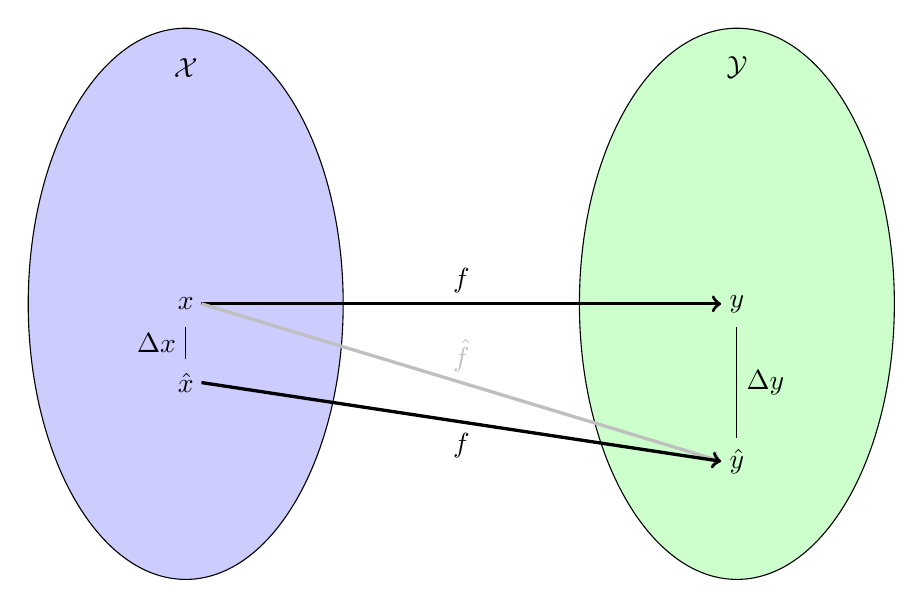
\begin{tikzpicture}
    \draw (0,0) ellipse (2cm and 3.5cm) [fill=blue!20];
    \draw (7,0) ellipse (2cm and 3.5cm) [fill=green!20];
    \draw (0,3)  node {$\mathcal{X}$};
    \draw (7,3)  node {$\mathcal{Y}$};
    \draw (0,0)  node {$x$};
    \draw (0,-1) node {$\hat{x}$}; 
    \draw (7,0)  node {$y$};
    \draw (7,-2) node {$\hat{y}$};
    \draw [->,very thick] (0.2,0) -- (6.8,0) node [midway,above] {$f$};
    \draw [->,very thick,black!25] (0.2,0) -- (6.8,-2) node [midway,above] {$\hat{f}$};
    \draw [->,very thick] (0.2,-1) -- (6.8,-2) node [midway,below] {$f$};
    \draw [-] (7,-0.3) -- (7,-1.7) node [midway,right] {$\Delta y$};
    \draw [-] (0,-0.3) -- (0,-0.7) node [midway,left] {$\Delta x$};
\end{tikzpicture}
\end{document}
